% The first command in your LaTeX source must be the \documentclass command.

\documentclass[sigconf]{acmart}
 % Do not change for ICTIR'19

\settopmatter{printacmref=true}
  % mandatory for ICTIR'19

\fancyhead{}
  % do not delete this code.
\usepackage{balance}
  % for creating a balanced last page (usually last page with references)
 %activate todo's
%\newcommand{\todo}[1]{\textcolor{red}{TODO: #1}\PackageWarning{TODO:}{#1!}}
% deactivate todos
%\newcommand{\todo}[1]{ \PackageWarning{TODO:}{#1!}}

% defining the \BibTeX command - from Oren Patashnik's original BibTeX documentation.
\def\BibTeX{{\rm B\kern-.05em{\sc i\kern-.025em b}\kern-.08emT\kern-.1667em\lower.7ex\hbox{E}\kern-.125emX}}
    
% Rights management information. 
% This information is sent to you when you complete the rights form.
% These commands have SAMPLE values in them; it is your responsibility as an author to replace
% the commands and values with those provided to you when you complete the rights form.
%
% These commands are for a PROCEEDINGS abstract or paper.

\copyrightyear{2019} 
\acmYear{2019} 
\acmConference[ICTIR '19]{The 2019 ACM SIGIR International Conference on the Theory of Information Retrieval}{October 2--5, 2019}{Santa Clara, CA, USA}
\acmBooktitle{The 2019 ACM SIGIR International Conference on the Theory of Information Retrieval (ICTIR '19), October 2--5, 2019, Santa Clara, CA, USA}
\acmPrice{15.00}
\acmDOI{10.1145/3341981.3344243}
\acmISBN{978-1-4503-6881-0/19/10}


% Submission ID. 
% Use this when submitting an article to a sponsored event. You'll receive a unique submission ID from the organizers
% of the event, and this ID should be used as the parameter to this command.
\acmSubmissionID{ictir094s}


% end of the preamble, start of the body of the document source.

\begin{document}

\fancyhead{}
  % do not delete this code.


% The "title" command has an optional parameter, allowing the author to define a "short title" to be used in page headers.
\title[Support Passage Retrieval]{Why does this Entity matter? Support Passage Retrieval for Entity Retrieval}


% The "author" command and its associated commands are used to define the authors and their affiliations.
% Of note is the shared affiliation of the first two authors, and the "authornote" and "authornotemark" commands
% used to denote shared contribution to the research.
\author{Shubham Chatterjee}
\email{sc1242@cs.unh.edu}
%\orcid{1234-5678-9012}
\affiliation{
 \institution{University of New Hampshire}
  \city{Durham}
 \state{New Hampshire}
}
\author{Laura Dietz}
\email{dietz@cs.unh.edu}
\affiliation{
 \institution{University of New Hampshire}
  \city{Durham}
 \state{New Hampshire}
}

%
% By default, the full list of authors will be used in the page headers. Often, this list is too long, and will overlap
% other information printed in the page headers. This command allows the author to define a more concise list
% of authors' names for this purpose.
%\renewcommand{\shortauthors}{Chatterjee and Dietz}

%
% The abstract is a short summary of the work to be presented in the article.
\begin{abstract}
Our goal is to complement an entity ranking with human-readable explanations of how those retrieved entities are connected to the information need. While related to the problem of support passage retrieval, in this paper, we explore two underutilized indicators of relevance: contextual entities and entity salience. The effectiveness of the indicators are studied within a supervised learning-to-rank framework on a dataset from TREC Complex Answer Retrieval. We find that salience is a useful indicator, but it is often not applicable. In contrast, although performance improvements are obtained by using contextual entities, using contextual words still outperforms contextual entities.
\end{abstract}

%
% The code below is generated by the tool at http://dl.acm.org/ccs.cfm.
% Please copy and paste the code instead of the example below.
%
%\begin{CCSXML}
%<ccs2012>
% <concept>
%<concept_id>10002951.10003317.10003338</concept_id>
%<concept_desc>Information systems~Retrieval models and ranking</concept_desc>
%<concept_significance>500</concept_significance>
%</concept>
%</ccs2012>
%<concept>
%<concept_id>10002951.10003317.10003325</concept_id>
%<concept_desc>Information systems~Information retrieval query processing</concept_desc>
%<concept_significance>300</concept_significance>
%</concept>
%\end{CCSXML}
%
%\ccsdesc[500]{Information systems~Retrieval models and ranking}
%\ccsdesc[300]{Information systems~Information retrieval query processing}
%

%
% Keywords. The author(s) should pick words that accurately describe the work being
% presented. Separate the keywords with commas.
% \keywords{joint query-entity-passage features, entity context neighbors, entity salience, entity context document}


%
% This command processes the author and affiliation and title information and builds
% the first part of the formatted document.
\maketitle

\section{Introduction}
\label{sec:Introduction}

Entity ranking is important for applications which seek either a particular entity or a list of entities, for example, entities involved in the \textit{Brexit} such as \textit{Theresa May}.  Several studies show that 40-70\% of all web searches target entities \cite{guo2009named,balog2018entity}. Such queries are best answered by giving the user a ranking of relevant entities. However, in addition to the ranking of entities, presenting a short passage to the user which tells them how or why the entity is related to the query may be more helpful since it helps users decide if they want to know more about the entity. Analogous to search snippets, we want to present a short passage that explains why the entity is relevant to the query.   We study the following task:

\textbf{Task:} Given a user's information need $Q$; an external system predicts a ranking of entities $E$. Our task is to, for every relevant entity $e_i \in E$, retrieve and rank $K$ passages $s_{ik}$ that explain why this entity $e_i$ is relevant for $Q$---we call these support passages henceforth. 

\bigskip
\noindent As an example, consider the following query-entity pair and the corresponding support passage:
\begin{quote}
\textbf{Query: } Unfree labour \\
\textbf{Entity: } Detention (imprisonment) \\
\textbf{Support Passage: } \\
Unfree labour is a generic or collective term for those work relations, especially in modern or early modern history, in which people are employed against their will by the threat of destitution, detention, violence (including death), lawful compulsion, or other extreme hardship to themselves or to members of their families.
\end{quote}



% You said this already. In this paper, study the problem of complementing an entity ranking with support passages. This task is useful whenever entities are displayed along with web search results, such as entity cards \cite{berntson2012providing}.



 The novel contribution of this work is a joint model of contextual entity and salience features to rank passages for a given query and entity. We compare our model to two baselines, one baseline retrieves passages for the query-entity pair using a compound query of the query and entity terms, the second baseline scores passages for the query-entity pair by the number of relevant entities (for the query) contained in the passage.
 
In addition to being relevant for $Q$, those support passages $s_{ik}$ should mention the entity $e_i$ in a salient way. Salient means that the entity is central to the passage. The salience of an entity can be predicted with the toolkit SWAT \cite{swat}. %(See Section \ref{sec: entity salience}).

%\section{Example: Entity Salience}
%\label{sec: entity salience}
For the query \textit{Brexit} and the entity \textit{Theresa May}  consider the following two passages:
\begin{quote}
\textbf{Passage 1: }  If Labour and the Conservatives fail to reach an agreement, MPs will face a series of votes on Brexit options, which could include another referendum. Theresa May has said her government stands ready to abide by the decision of the House  if Labour does the same.\\
\textbf{Passage 2: } British Prime Minister Theresa May offered a new Brexit plan on Tuesday, in a last-ditch effort to get her still-unpopular Brexit deal approved.
\end{quote}

While both passages mention \textit{Theresa May} and are about \textit{Brexit}, Passage 2 discusses how Theresa May is affecting Brexit and hence the entity is central to the passage whereas in Passage 1 it is not.

%We notice that both passages mention the entity Theresa May and is about the query \textit{brexit}.However, in Passage 1 Theresa May is not central, whereas in Passage 2 it is (the passage talks about how Theresa May is affecting brexit).  This is an example of a good support passage, one which not only mentions the entity and makes a connection between the query-entity pair, but also mentions the entity in a salient, that is, central way. 
%\todo{since you have some space, I would explain what entity salience means or does not mean. It is likely that the reviewer does not know it. (yes, shocking!) SO if you spend 1 paragraph, maybe one picture with two examples following the brexit / Theresa may will be good.}


We develop a range of features which incorporate the salience of the entity in the passage for the task of support passage retrieval. We explore if predictions made by SWAT are sufficient to reap the benefits from entity salience. The effectiveness is evaluated in a learning-to-rank \cite{liu2009learning} setting.\footnote{For more experiments, results, descriptions of methods and datasets, refer to the online appendix for this paper at:  \url{https://shubham526.github.io/support-passage-retrieval/.}}


%Our hypothesis is that incorporating entity salience should help; in this work we study if we have the necessary tools to reap benefits from entity salience. The issues our study reveals are not due to failures of the salience detection model, but because the retrieval models available today are not modelling salience, and therefore passages in the pool do not mention the entity in salient ways. 




\section{Related Work}
\label{sec:related work}
%\paragraph{\textbf{Sentence Retrieval}}
Sentence Retrieval retrieves relevant sentences in response to a query, question or another sentence. Tasks such as question answering \cite{cardie2000examining}, summarization, novelty detection, topic detection and tracking \cite{stokes2001first}, and information provenance make use of a sentence retrieval module as a pre-processing step. However, none of these address the task of support sentence retrieval. The closest is perhaps the work by Cardie et al.\ \cite{cardie2000examining} which discusses sentence ranking models where the query includes a constraint on a type of entity(e.g. a location, a person). 
Blanco and Zaragoza \cite{blanco2010finding} present a model that ranks entity support sentences with learning-to-rank. Their work focuses on features based on named entity recognition (NER) in combination with term-based retrieval models. 
%\paragraph{\textbf{Entity Relation Explanation}}

Voskarides et al.\ \cite{voskarides2015learning} study the problem of explaining relationships between pairs of knowledge graph entities with human-readable descriptions. They model the task as a learning-to-rank problem with a rich set of features which include textual, entity and relationship features. Aggarwal et al.\ \cite{aggarwal2016connecting} rank all the paths between any two entities in a knowledge graph. This can help in explaining relationships between seemingly unconnected entities. 

%\paragraph{\textbf{Support Passage Retrieval}}
Kadry and Dietz \cite{kadry2017open} use relation extraction using OpenIE for support passage retrieval. Their work studies how relation extraction can help in support passage retrieval and the limitations of the current relation extraction approaches that need to be overcome. Their work explores a rich set of features for our task.  

None of the works above study joint query-entity and paragraph relevance nor do they consider the effect of entity salience. We propose to look at features that model the joint relevance of a paragraph to an entity and a query, which captures the entity salience in the passage. 


\section{Approach}
\label{sec:approach}
%  not needed: \subsection{Overview}
%\label{subsec:overview}
Given a ranked list of entities for a query, we seek to embellish it with passages which would explain to the user why the entity is relevant to the query. We call the entities in the ranking as target entities. We only try to predict support passages for target entities which are also relevant (according to the entity ground truth for the query). To model this joint relevance for \textit{both} the query and the entity, we use the co-occurring entities with a given entity. 

\subsection{Candidate Passage Generation}
\label{subsec:candidate passage generation}
We generate the candidate set of passages using a learning-to-rank combination of the following retrieval models. The RM1/RM3 are expanding with words in this case. Later, we also use RM1/RM3 for expanding the query with entities. 
%\todo{Make clear that your RM3/RM1 is expanding with words. Later you are expanding with entities (expanding wth entities is something I like to do, but its not usual in the community}:
\begin{itemize}
    \item BM25 (default Lucene) with RM1 (BM25 + RM1)
    \item BM25 (default Lucene) with RM3 (BM25 + RM3)
    \item Language Models with Jelinek-Mercer smoothing $(\lambda = 0.4)$, with RM1 (LMJM + RM1)
    \item Language Models with Jelinek-Mercer smoothing $(\lambda = 0.4)$, with RM3 (LMJM + RM3)
    \item Language Models with Dirichlet smoothing, with RM1 (LMDS + RM1)
    \item Language Models with Dirichlet smoothing, with RM3 (LMDS + RM3)
\end{itemize}


\subsection{Features}
\label{subsec:features}
\subsubsection{Features based on co-occurring entities}
\label{subsubsec:features:1}
We assume that a passage with a lot of query-relevant entities which co-occur frequently with a given entity is likely talking about that entity. To find most frequently co-occurring entities with a given entity, we filter all passages (retrieved for the query) mentioning the entity and "stitch" them together into $D_e$ which we call an \textit{Entity Context Document} (ECD) about the entity $e$, following an idea of Dalton et al.\ \cite{dalton2014entity} (Figure \ref{fig:pseudo-doc}). 
All entities $e' \in D_e$ co-occur with $e$. A distribution over these co-occurring entities would tell us how likely we are to see the co-occurring entity $e'$ provided we have already seen the query-entity pair $(q, e)$. We derive this distribution by finding the number of times an entity $e'$ occurs in the ECD. More formally, 

\begin{equation}
\label{eq:1}
    P(e'|e,q) \propto \sum_{p \in D_e} count(e'\in p)
\end{equation}
where $p$ is a paragraph, $D_e$ is the ECD about entity $e$, $e' (\ne e)$ is an entity co-occurring with $e$, and $count(e')$ is the number of times $e'$ is mentioned in $p$. 

\begin{enumerate}
    \item \textbf{Entities in the Entity Context Neighbors (ECN).} \label{en:entity context neighbors} We score a passage in an ECD $D_e$ by accumulating co-occurrence scores of entities $e'$ contained therein. 
More formally, we can define a feature value $f_{qe}(p)$ of a paragraph $p \in D_e$ for query-entity pair $(q, e)$ as
\begin{equation}
\label{eq:2}
    f_{qe}(p) = \sum_{e' \in p} P(e'|e,q)
\end{equation}
\begin{figure}
 \centering 
 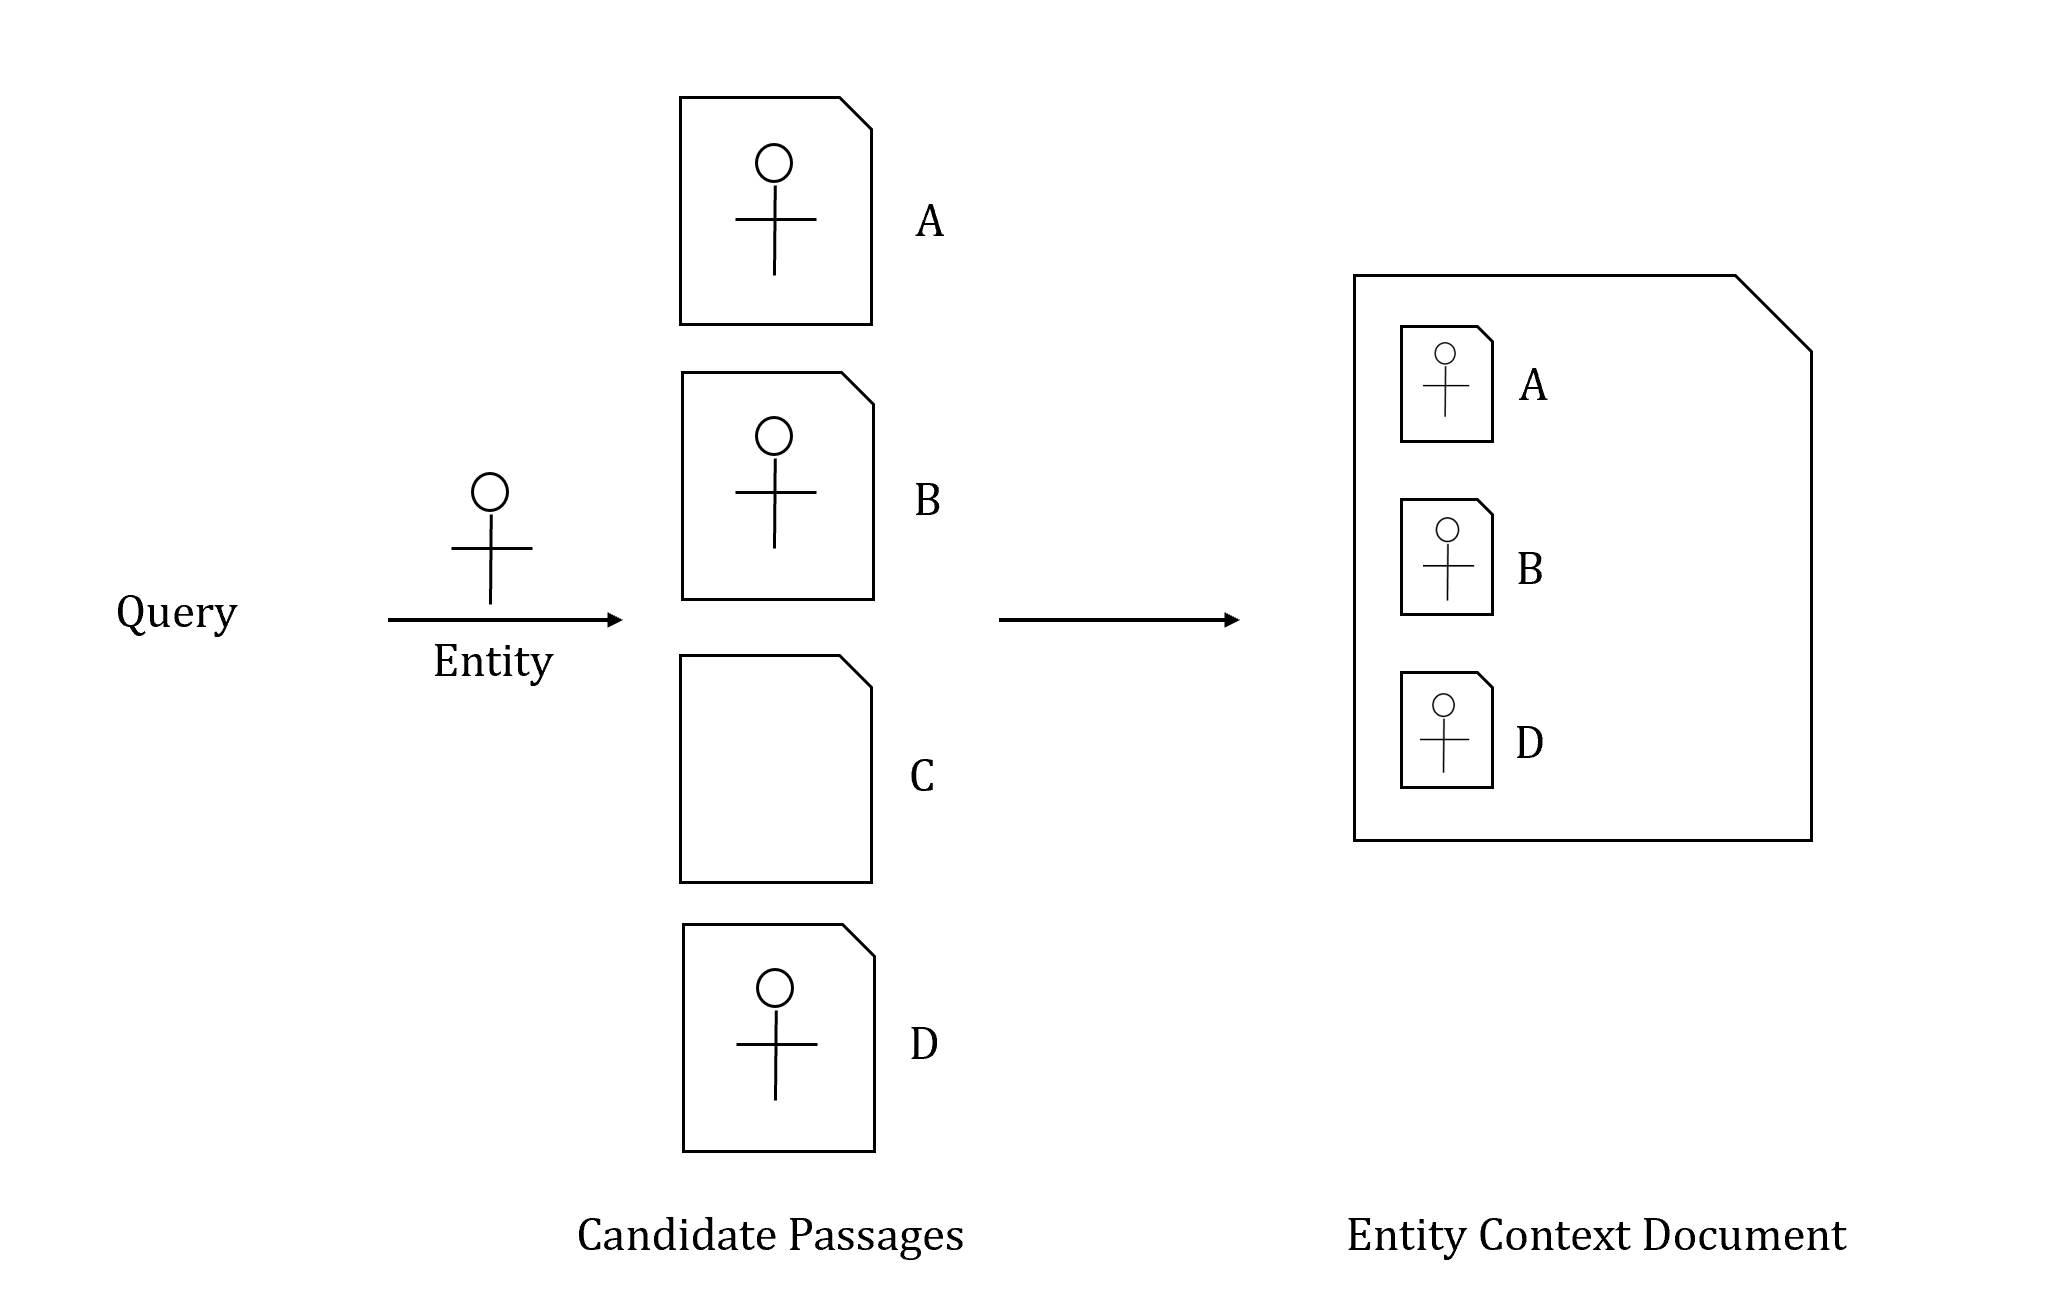
\includegraphics[scale=0.44]{ecd.PNG}
 \caption{Entity Context Document}
 \label{fig:pseudo-doc}
\end{figure}
\item \textbf{Query expansion using entities (QEE) from ECD.} \label{en: Query expansion using entities from entity context documents} Using top 20 co-occurring entities to expand the query using RM1 and RM3 on a search index that has a separate field for entities. We experiment with the same variations as given in Section \ref{subsec:candidate passage generation}. Each variation becomes a feature.
\end{enumerate}
\subsubsection{Features based on entity context documents}
\label{subsubsec:feature:2}
\begin{enumerate}
    \item \textbf{Retrieval score of an ECD.} \label{en:Retrieval score of a entity context document}For every query, we retrieve ECDs using BM25. There is one ECD per entity consisting of passages mentioning the entity. A passage might mention several entities and hence may be present in the ECD of more than one entity. 
    As in Section \ref{subsubsec:features:1} (\ref{en:entity context neighbors}), we obtain a passage score by accumulating the scores of the ECDs it appears in. 

    \item \textbf{Query expansion using words (QEW) from ECD.} \label{en:Query expansion using words from entity context document} Similar to Section \ref{subsubsec:features:1} (\ref{en: Query expansion using entities from entity context documents}), we expand the query using terms from the ECDs using pseudo relevance feedback. We use top 50 terms for expansion and 100 documents as the feedback set. We experiment with the same variations as given in Section \ref{subsec:candidate passage generation}. Each variation becomes a feature.
\end{enumerate}

\subsubsection{Features based on entity salience}
\label{subsubsec:feature:3}
We use SWAT \cite{swat} to annotate passages with salient entities and salience score and class (whether salient or not). We consider $\text{Score}(p \vert e)$ = $\text{Salience}(e \vert p)$. We score a passage $p$ for the query-entity pair $(q,e)$ in two ways: 

\begin{enumerate}
    \item \textbf{Salience score of passage with co-occurring entities
    (SSP-CE).} We obtain a support passage ranking for every query-entity pair from the method in \ref{subsubsec:features:1}(\ref{en:entity context neighbors}). We re-rank these passages using 
    \begin{equation}
        \label{eq:3}
            \text{Score}(p \vert e, q) =  \text{Score}(p \vert e) \cdot \text{Score}(e \vert q)
    \end{equation}
 where $\text{Score}(e \vert q)$ is the normalized retrieval score of $e$ (obtained from the entity ranking) and $\text{Score}(p \vert e)$ is the normalized salience score of $e$ for $p$.
    
    \item \textbf{Salience score of passage which mentions an entity
    (SSP-EM).}
    %passage in a entity context document} 
    We obtain an ECD about an entity and rank the passages in this ECD using
    \begin{equation}
        \label{eq:4}
            \text{Score}(p \vert e, q) =  \text{Salience}(e \vert p) \cdot \text{Score}(p \vert q)
    \end{equation}
 where $\text{Score}(p \vert q)$ is the normalized retrieval score of $p$ (obtained from the candidate passage ranking) and $\text{Salience}(e \vert p)$ is the normalized salience score of $e$ for $p$.
\end{enumerate}
\section{Evaluation}
\label{sec:Evaluation}
\subsection{Research Questions}
\label{subsec:research questions}
We study the extent to which the following components in our approach affect the quality of retrieved support passages:

\begin{itemize}
\item[\textbf{RQ1}] What is the effect of contextual entities?
\item[\textbf{RQ2}] What is the effect of entity salience? 
\item[\textbf{RQ3}] Is it better to expand queries with entities or words?
\end{itemize}

%Our goal is to study the following research questions.\\
%\textbf{RQ1} To what extent do entities in context affect the support passage retrieval?  \\\\
%\textbf{RQ2} To what extent does entity salience affect the support passage retrieval?  \\
%\textbf{RQ3} Are contextual entities more informative than contextual words? 


\subsection{Evaluation Paradigm}
\label{subsec:Evaluation Paradigm}
We use the dataset from the TREC Complex Answer Retrieval track \cite{dietz2017trec}\footnote{\url{http://trec-car.cs.unh.edu}} to evaluate our methods. It contains both passage and entity ground truth data as well as an entity linked corpus consisting of paragraphs from the entire English Wikipedia. We use the entity links provided in the collection as well as those annotated using TagMe \cite{ferragina2010tagme}. We derive a ground truth for entity support passage retrieval from the ground truth of relevant passages and entities provided with the data set (article-level) as follows: any relevant passage that contains an entity link to a relevant entity for the query is defined as relevant for the given query and entity. We apply our methods to produce a passage ranking for every query-entity pair and perform 5-fold cross validation. We use RankLib\footnote{Dang, V. "The Lemur Project-Wiki-RankLib." Lemur Project,[Online]. Available: \url{http://sourceforge. net/p/lemur/wiki/RankLib}.} with Coordinate Ascent
to optimize for Mean Average Precision (MAP). We use MAP, Mean Reciprocal Rank (MRR), Precision at R (P@R) and Precision at 1 (P@1) as our evaluation metrics---omitted results are available in our online appendix.   
\subsection{Baseline}
\label{subsec:Baseline}
We include two baselines that use query and entity, without any other components of our approach.

\subsubsection{Baseline 1: Frequency of relevant entity links} 

\label{subsubsec: baseline 1}
We rank passages for a query-entity pair by the number of relevant entities in the passage. For example, if a passage $p$ contains entities $\{e_1,e_2\}$ and the entities $\{e_1,e_2,e_3,e_4\}$ have been retrieved for the query $q$, then the score of $p$ for each of the query-entity pairs is $f_{qe_1}(p)=f_{qe_2}(p)=2$ because the passage has two entities in common with the list retrieved for $q$.

\subsubsection{Baseline 2: Compound entity-query score} 
\label{subsubsec: baseline 2}
We retrieved passages using a compound query, where the query is a combination of the original query and the target entity. 
\subsection{Results}
\label{subsubsec: reults}
\begin{table}
  \caption{Performance with standard error of features individually and combined with L2R, including subsets/ablations.}
  \label{tab:results}
  %\scalebox{1.1}{
  \begin{tabular}{lp{2cm}p{2cm}l}
  
    \toprule
    
    & MAP & P@1 
    \\
    
    \midrule
    
    Baseline 1&	
    0.09$\pm$0.002&		
    0.06$\pm$0.002 
    \\
    
    Baseline 2&	
    0.07$\pm$0.003&	
    0.06$\pm$0.003 
    \\
    
    \midrule
    
    ECN & 
    0.31$\pm$0.004 & 
    0.30$\pm$0.004 
    \\

    %\midrule
    
    QEW (LMJM+RM3)&	
    0.35$\pm$0.004&	
    0.34$\pm$0.004 
    \\
    
    %\midrule

    QEE  (LMJM+RM3)&	
    0.30$\pm$0.003&	
    0.28$\pm$0.004 
    \\
    
    %\midrule
    
    SSP-CE&
    0.01$\pm$0.002&	
    0.02$\pm$0.003 
    \\

    SSP-EM&
    0.02$\pm$0.003&	
    0.03$\pm$0.004 
    \\

    \midrule

    L2R-All-Features& 
    0.30$\pm$0.004&	
    0.34$\pm$0.004 
    \\
    
    \midrule
    
    Subset-1 (all $-$ QEW)&	
    0.28$\pm$0.004& 
    0.30$\pm$0.004&
    \\	
    
    Subset-2 (all $-$ QEE)&	
    0.35$\pm$0.004&
    0.35$\pm$0.004&
    \\
    
    %Subset-3&	
    %0.35$\pm$0.004&
    %0.34$\pm$0.004&
    %\\	
    
    Subset-3 (only QEW)&	
    0.35$\pm$0.004&
    0.34$\pm$0.004&
    \\
    
    Subset-4 (only QEE)&	
    0.30$\pm$0.004&
    0.29$\pm$0.004
    \\
    
    Subset-5 (QEW $+$ QEE)&	
    0.35$\pm$0.004&
    0.34$\pm$0.004
    \\

    \bottomrule
\end{tabular}
%}
\end{table}

The most interesting results are presented in Table \ref{tab:results}. Due to space contraints other results were moved to the online appendix for this paper. Below, we discuss each of the research questions presented in Section \ref{subsec:research questions}.

\textbf{RQ1 (contextual entities):} We observe in Table \ref{tab:results} that ranking passages with contextual entities (ECN) achieves a MAP of 0.31 and query expansion with entities (QEE) a MAP of 0.30. This is a significant improvement over the two baselines which have a MAP of 0.09 and 0.07 respectively. This demonstrates the benefit of contextual entities. See Section \ref{subsec: ablation_study} for more discussion.

\textbf{RQ2 (entity salience):} We observe in Table \ref{tab:results} that the two methods which rank passages using entity salience perform the worst. This is also the case when combined with other features using learning-to-rank. We manually confirmed that SWAT correctly identifies salient and non-salient entities.  However, only few retrieved entities have a passage with a salient mention. While entities with salient passages are often relevant, a majority (95\%) of retrieved entities do not have a passage with a salient mention in the candidate pool. Since the salience feature is only applicable to very few entities, it only has a limited impact on the overall result. 

%Hence, we need better candidate pool because BM25, Query Likelihood, Relevance Model did not include the entity during retrieval, and do not have any notion of salience. % I am not sure this statement is true, but we can omit if from the text and its fine.

To study whether salience is a useful indicator when it is applicable, we analyze results on the subset of rankings for query-entity pairs for which the passage ranking contains at least one passage in which the target entity %\todo{target entity?} 
is salient. The results are shown in Table \ref{tab:salience results}. We observe that the salience indicator performs very well as compared to other methods. Hence, salience is a useful indicator---however it is only applicable for entities which have a salient passage in the candidate pool.
(More results in the online appendix.)
\begin{table}
  \caption{ Results on subset of entities with at least one salient mention.}
  \label{tab:salience results}
  %\scalebox{0.6}{
  \begin{tabular}{lp{2cm}p{2cm}l}
  
    \toprule
    
    & MAP & P@1 \\
    
    \midrule
    
    Baseline 1&	
    0.16$\pm$0.01&	
    0.12$\pm$0.01 \\
    
    Baseline 2&	
    0.09$\pm$0.01&	
    0.10$\pm$0.01 \\
    
    \midrule
    
    ECN& 
    0.41$\pm$0.02& 
    0.37$\pm$0.02 \\
    
    \midrule
    
    SSP-CE&	
    0.47$\pm$0.02&	
    0.64$\pm$0.02 \\

    SSP-EM&	
    0.28$\pm$0.01&	
    0.40$\pm$0.02 \\

\bottomrule
\end{tabular}
%}
\end{table}

\textbf{RQ3 (query expansion):} We observe that among all methods which retrieve with contextual entities, the method using LMJM with RM3 performs the best with a MAP of 0.30. Note that here we use RM3 to expand the query with entities (see Section \ref{subsubsec:features:1}(\ref{en: Query expansion using entities from entity context documents})). Also, among all methods which retrieve with contextual words, the methods using LMJM with RM3 performs the best with a MAP of 0.35.  As we can see, retrieval with contextual words outperforms retrieval with contextual entities and although contextual entities achieve good results, they are unable to outperform contextual words.  Hence, contextual words are more informative than contextual entities. Another observation is that among BM25, LMDS and LMJM, retrieval with LMJM always gives the best performance for both contextual entities and contextual words. For more discussion, see Section \ref{subsec: ablation_study}.

\subsection{Subset Ablation Study}
\label{subsec: ablation_study}
From Table \ref{tab:results} we observe that using QEW features alone obtain a higher MAP score than learning-to-rank with all features. To investigate this further, we conduct a subset/ablation study using learning-to-rank with 5-fold cross-validation using the following combinations:. 

\begin{enumerate}
    \item \textbf{Subset-1}: All features except QE with word features.
    \item \textbf{Subset-2}: All features except QE with entities features.
    %\item \textbf{Subset-3}: All features except \textit{Entity Context Neighbors} and \textit{Retrieval Score of Entity Context Document}
    \item \textbf{Subset-3}: Only QE with word features.
    \item \textbf{Subset-4}: Only QE with entity features.
    \item \textbf{Subset-5}: Only QE with entity and QE with word features.
    
\end{enumerate}
The results are shown at the bottom of Table \ref{tab:results}.
%We observe that although the combination all variations of QE with entity features (Subset-4) performs well on its own, mixing them with other features reduces the MAP from 0.35 on subset-2 to 0.30 on all features.

Regarding RQ1, we observe that although the combination all variations of QEE with entity features (Subset-4) performs well on its own, the ablation study shows that  one would obtain even better results by leaving QEE features out (Subset-2) to improve to a MAP 0.35.
%
In contrast, QEW with word features (Subset-3) performs well on their own as well as in the mix with other features as is evident by an increase in MAP of 0.28 on Subset-1 to MAP of 0.30 on all. Hence, we conclude that contextual entities affect the support passage retrieval to a lesser extent than contextual words.

%\todo{We need to discuss P@1 here, see my email}

Regarding RQ3, when L2R is trained to optimize MAP on all contextual word and entity features (Subset-5) the trained parameter assigns the maximum weight to contextual word features (in particular, QE with word using LMJM and RM1/RM3). This shows that contextual words are more informative than contextual entities.

%Hence, we conclude that although we can obtain performance improvements over the baselines using methods which use contextual entities to rank support passages, using contextual words still outperforms contextual entities and are more informative. 
%We observe that a learning-to-rank combination of all features except the QE with entity features (subset-2) achieves a significant improvement over the learning-to-rank combination of all features and that a learning-to-rank combination of only QE with entity features (subset-5) performs well. This shows that although subset-5 features perform well on their own, they do not mix well with all the features. We also observe that the performance of all features except QE with word features (subset-1) drops as compared to learning-to-rank combination of all features and that the QE with word features (subset-4) perform well on their own. This shows that subset-4 features perform well on their own and mix well with other features to boost the MAP score. From the results we can see that contextual words affect support passage retrieval to a greater extent than contextual words. We also observed that the weights assigned by Coordinate Ascent to the features in subset-4 are equal whereas those assigned to features in subset-5 are not. This shows that all the subset-4 features give the same information and contextual entities are indeed more informative than contextual words. (RQ3)
\section{Conclusion and Future Work}
\label{sec: conclusion}
This work addresses the task of support passage retrieval to enrich entity rankings in response to a search query. We propose a joint query-entity-passage ranking method and present some initial results. In particular, we show that co-occurring entities are an important indicator of which passages might support an entity for a query. In contrast, retrieving passages using a compound query of the original query and the entity is not sufficient for the problem.

We also experiment with entity salience, and find that it is a highly informative feature when it is applicable, however 95\% of target entities do not have any passage with a salient mention in the candidate set. We thus identify a need for developing high-recall salience techniques that are applicable to a larger number of entities, as well as new indexing and retrieval methods that integrate entity salience in an early phase.
%As future work, it would be interesting to see how incorporating salience while constructing the entity entity context documents affects the performance and how expanding with salient entities performs.

%
% The next two lines define the bibliography style to be used, and the bibliography file.
%\begin{acks}
%We would like to thank everyone who gave useful insights to improve the paper and helped to make it more readable. In particular, we would like to thank Jordan Ramsdell from the TREMA lab at UNH who gave many useful insights into the problem and helped to polish it further. We would also like to thank the Graduate School at the University of New Hampshire for providing a travel grant to attend the conference.
%\end{acks}
\bibliographystyle{ACM-Reference-Format}
\bibliography{bibliography}
% If your work has an appendix, this is the place to put it.

%\appendix
%\section{Online Resources}
%For more experiments, results, descriptions of methods and datasets, refer to the online appendix for this paper at:  \url{https://shubham526.github.io/support-passage-retrieval/.}
\end{document}
